The parameters within the two models were identified with inverse dynamics regression (ID regression) on a set of manoeuvring model tests conducted with a scale model of the WPCC. All of the zigzag10/10, and zigzag20/20 model tests to port and starboard were included in the training dataset to identify the parameters within the Abkowitz and the Physics informed model.
%\begin{figure}[h]
%    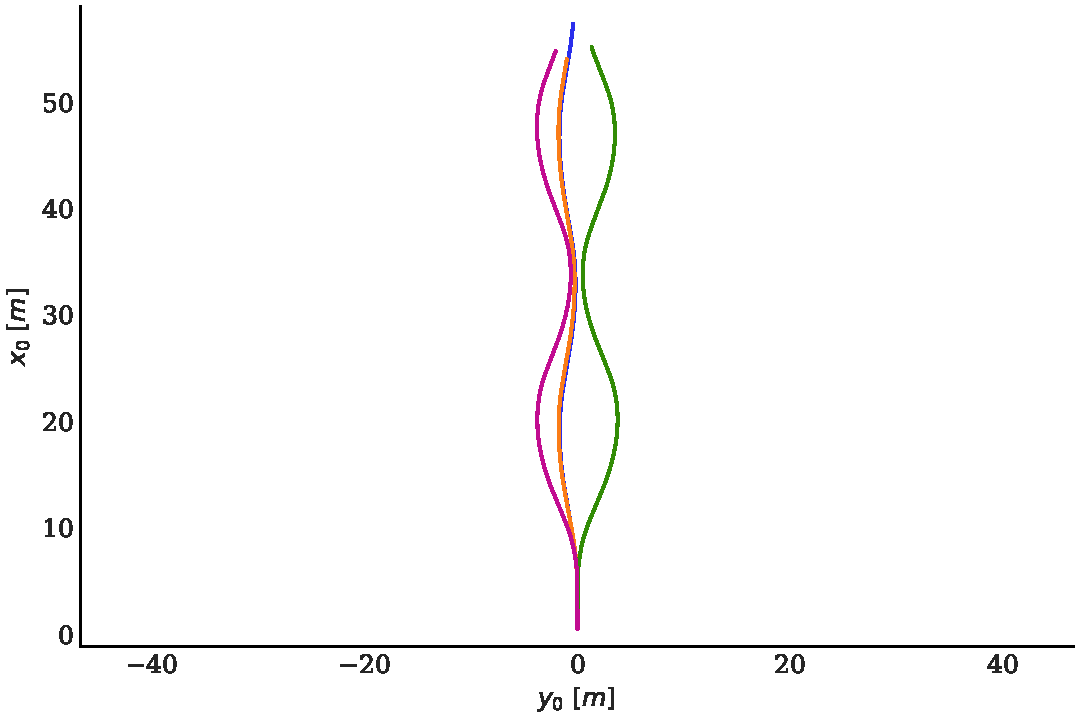
\includegraphics[width=\columnwidth]{figures/result_ID_regression.model_tests.pdf}
%    \caption{Model tests trajectories.}
%    \label{fig:model_tests}
%\end{figure}

\autoref{fig:ID_regression_ID_N} shows the yawing moments for one of the zigzag20/20 tests predicted with the models. The yawing moment from the zigzag experiment, estimated with inverse dynamics, has also been added to these graphs -- as a second reference of the total forces. It seems that the the yawing moments are similar for all models and the experimental data. It can also be seen that the Reference model and Semi-empirical ID predicts the exact same rudder yawing moment $N_R$, since they both use the same deterministic semi-empirical rudder model -- the yawing moments from the hull $N_H$ are therefore similar for these models. The rudder yawing moment from the Abkowitz ID is however very different. The regression has thus been forced to also make the yawing moments from the hull $N_H$ to be very different -- so that the total yawing moment adds up to be correct. This means that the total yawing moment is the same for all models, but the decomposition to hull and rudder moments turns out to be very different.
%\begin{figure}[h!]
%    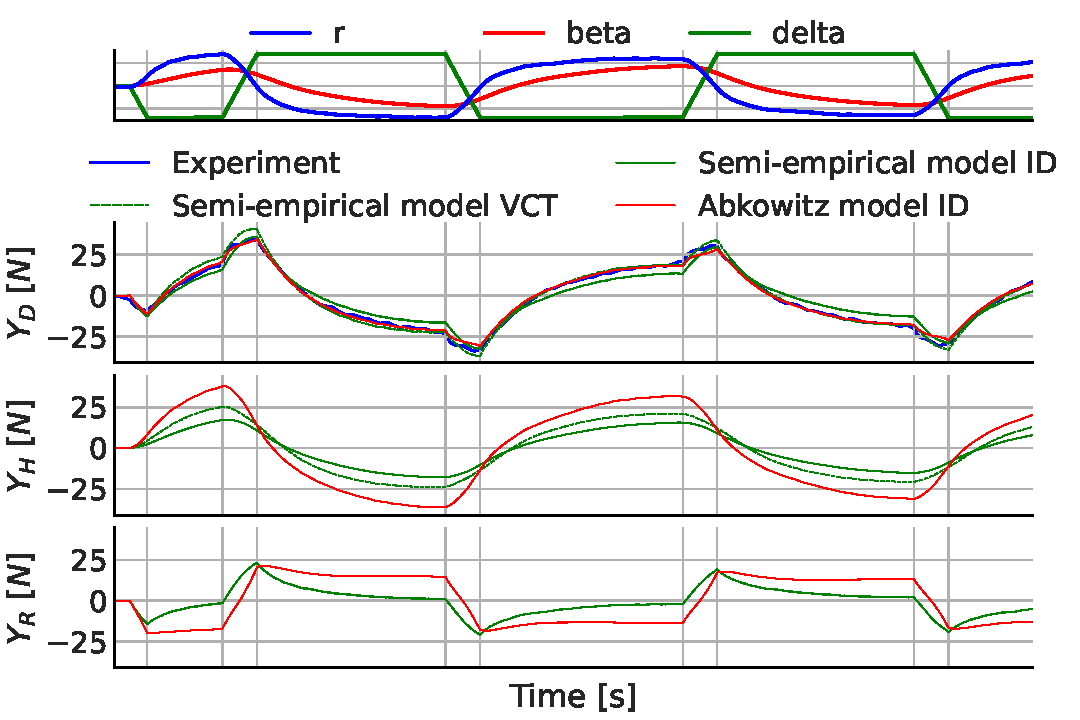
\includegraphics[width=\textwidth]{figures/result_ID_regression.ID_regression_ID_Y.pdf}
%    \caption{}
%    \label{fig:ID_regression_ID_Y}
%\end{figure}
\begin{figure}[h]
    \centering
    \includesvg[width=\columnwidth]{figures/results.ID_zigzag20.svg}
    \caption{Comparison of the total yawing moment acting on the ship: predicted with the Semi-empirical VCT model, predicted with the Semi-empirical ID model, predicted with the Abkowitz ID model, and the corresponding values from a zigzag20/20 test estimated with inverse dynamics.}
    \label{fig:ID_regression_ID_N}
\end{figure}
\autoref{fig:ID_models_mean_average_error} shows mean average prediction error for all of the the model tests. The models have about the same error in surge force $X_D$, and yawing moment $N_D$, but the Abkowitz model sway force error is much lower than the Physics informed model. 
\begin{figure}[h]
    \begin{center}
        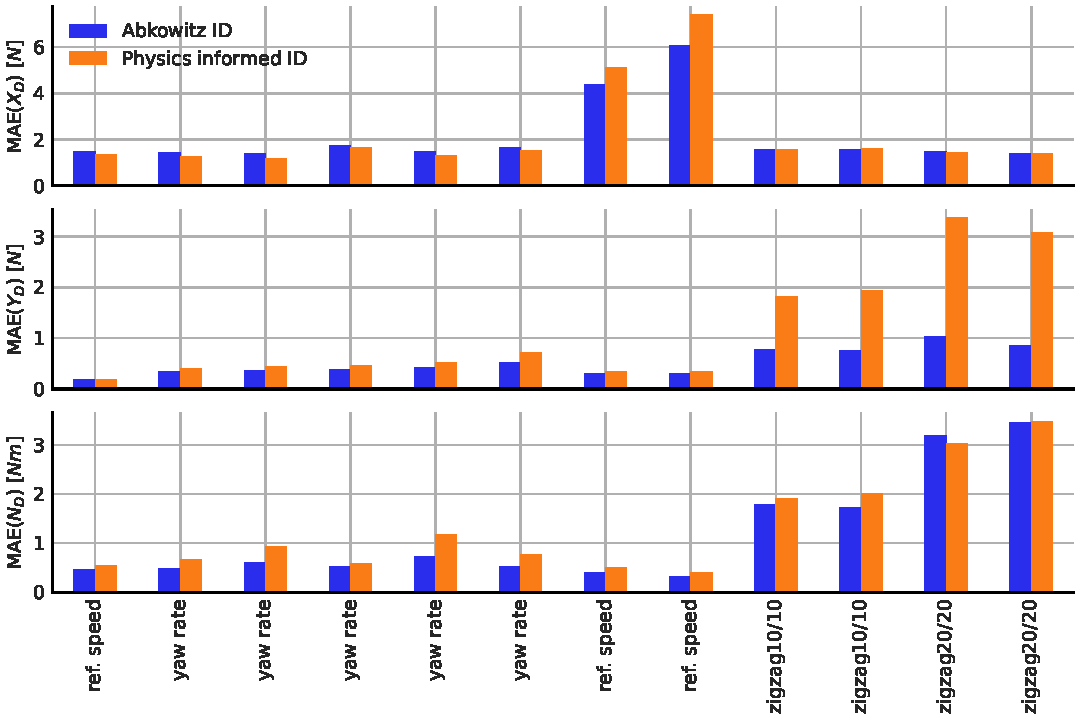
\includegraphics[width=\columnwidth]{figures/result_ID_regression.ID_models_mean_average_error.pdf}
        \caption{Mean average error of the models compared to the inverse dynamics
forces from the rest of the models tests.}
        \label{fig:ID_models_mean_average_error}
    \end{center}
\end{figure}

The hull force model can be closer examined by decomposing the individual parameter contributions. \autoref{fig:ID_regression_N_decomposition} shows the parameter decomposition for the two models together with the Reference model. The graphs show the joined contributions for parameters related to drift ($N_v+N_{vvv}$), yaw rate ($N_r+N_{rrr}$), and combined drift and yaw rate ($N_{vrr}+N_{vvr}$). It seems that Semi-empirical ID has similar parameter decomposition to the Reference model with the exception of $N_{vrr}+N_{vvr}$ being very small; it seems that $N_r+N_{rrr}$ are a little bit larger to compensate.
The parameter decomposition of the Abkowitz ID is completely different, where almost the entire contribution to the hull yawing moment $N_H$ can be denoted to the yaw rate parameters $N_r+N_{rrr}$. 
\begin{figure}[h]
    \begin{center}
        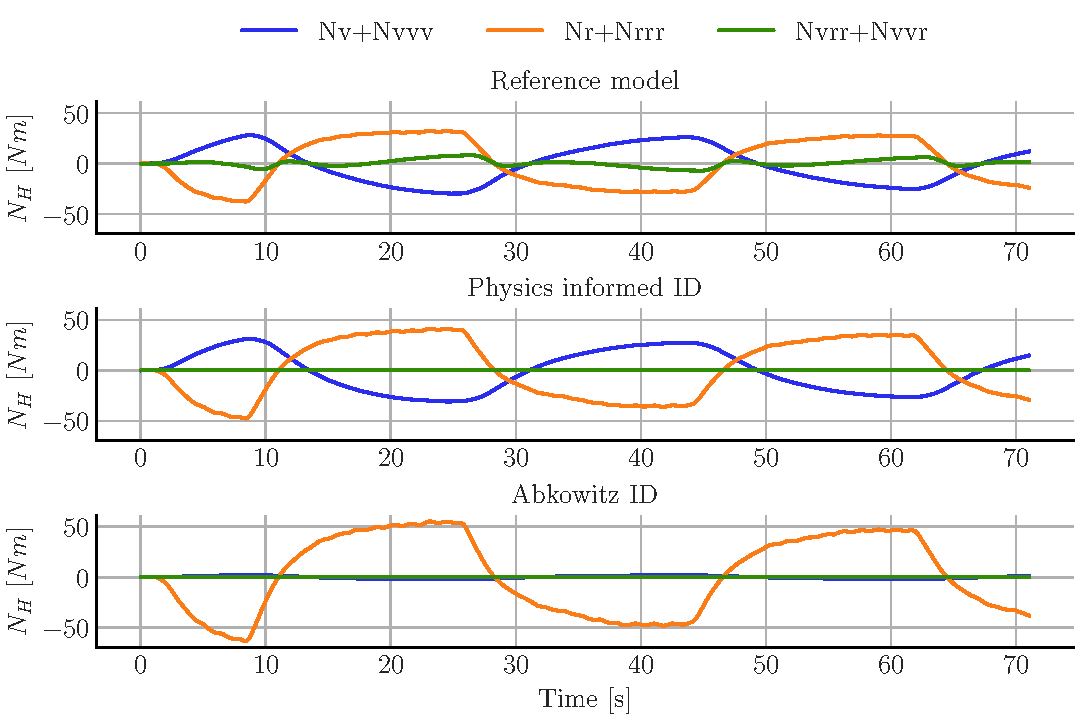
\includegraphics[width=\columnwidth]{figures/result_ID_regression.ID_regression_N_decomposition.pdf}
        \caption{Parameter contributions to the hull forces during a zigzag20/20 test for parameters related to drift, yaw rate and combined drift and yaw rate for the three prediction models.}
        \label{fig:ID_regression_N_decomposition}
    \end{center}
\end{figure}

Possible implications of that the Abkowitz model have this physically incorrect decomposition of the hull's drift angle and yaw rate dependence will be further investigated in the next section.
